%%%%%%%%%%%%%%%%%%%%%%%%%%%%%%%%%%%%%%%%%
% Lachaise Assignment
% LaTeX Template
% Version 1.0 (26/6/2018)
%
% This template originates from:
% http://www.LaTeXTemplates.com
%
% Authors:
% Marion Lachaise & François Févotte
% Vel (vel@LaTeXTemplates.com)
%
% License:
% CC BY-NC-SA 3.0 (http://creativecommons.org/licenses/by-nc-sa/3.0/)
% 
%%%%%%%%%%%%%%%%%%%%%%%%%%%%%%%%%%%%%%%%%

%----------------------------------------------------------------------------------------
%	PACKAGES AND OTHER DOCUMENT CONFIGURATIONS
%----------------------------------------------------------------------------------------

\documentclass{article}
\usepackage{amsthm}
\usepackage{listings}
\usepackage{xcolor}
\usepackage{graphicx}
\usepackage{float}


\lstset{
	language=Python,
	basicstyle=\ttfamily\small,
	keywordstyle=\color{blue},
	stringstyle=\color{red},
	commentstyle=\color{purple},
	showstringspaces=false,
	numbers=left,
	numberstyle=\tiny\color{gray},
	breaklines=true,
	frame=single,
	captionpos=b
}
\newtheorem{definition}{Definition}[section]

%%%%%%%%%%%%%%%%%%%%%%%%%%%%%%%%%%%%%%%%%
% Lachaise Assignment
% Structure Specification File
% Version 1.0 (26/6/2018)
%
% This template originates from:
% http://www.LaTeXTemplates.com
%
% Authors:
% Marion Lachaise & François Févotte
% Vel (vel@LaTeXTemplates.com)
%
% License:
% CC BY-NC-SA 3.0 (http://creativecommons.org/licenses/by-nc-sa/3.0/)
% 
%%%%%%%%%%%%%%%%%%%%%%%%%%%%%%%%%%%%%%%%%

%----------------------------------------------------------------------------------------
%	PACKAGES AND OTHER DOCUMENT CONFIGURATIONS
%----------------------------------------------------------------------------------------

\usepackage{amsmath,amsfonts,stmaryrd,amssymb} % Math packages

\usepackage{enumerate} % Custom item numbers for enumerations

\usepackage[ruled]{algorithm2e} % Algorithms

\usepackage[framemethod=tikz]{mdframed} % Allows defining custom boxed/framed environments

\usepackage{listings} % File listings, with syntax highlighting
\lstset{
	basicstyle=\ttfamily, % Typeset listings in monospace font
}

%----------------------------------------------------------------------------------------
%	DOCUMENT MARGINS
%----------------------------------------------------------------------------------------

\usepackage{geometry} % Required for adjusting page dimensions and margins

\geometry{
	paper=a4paper, % Paper size, change to letterpaper for US letter size
	top=2.5cm, % Top margin
	bottom=3cm, % Bottom margin
	left=2.5cm, % Left margin
	right=2.5cm, % Right margin
	headheight=14pt, % Header height
	footskip=1.5cm, % Space from the bottom margin to the baseline of the footer
	headsep=1.2cm, % Space from the top margin to the baseline of the header
	%showframe, % Uncomment to show how the type block is set on the page
}

%----------------------------------------------------------------------------------------
%	FONTS
%----------------------------------------------------------------------------------------

\usepackage[utf8]{inputenc} % Required for inputting international characters
\usepackage[T1]{fontenc} % Output font encoding for international characters

\usepackage{XCharter} % Use the XCharter fonts

%----------------------------------------------------------------------------------------
%	COMMAND LINE ENVIRONMENT
%----------------------------------------------------------------------------------------

% Usage:
% \begin{commandline}
%	\begin{verbatim}
%		$ ls
%		
%		Applications	Desktop	...
%	\end{verbatim}
% \end{commandline}

\mdfdefinestyle{commandline}{
	leftmargin=10pt,
	rightmargin=10pt,
	innerleftmargin=15pt,
	middlelinecolor=black!50!white,
	middlelinewidth=2pt,
	frametitlerule=false,
	backgroundcolor=black!5!white,
	frametitle={Command Line},
	frametitlefont={\normalfont\sffamily\color{white}\hspace{-1em}},
	frametitlebackgroundcolor=black!50!white,
	nobreak,
}

% Define a custom environment for command-line snapshots
\newenvironment{commandline}{
	\medskip
	\begin{mdframed}[style=commandline]
}{
	\end{mdframed}
	\medskip
}

%----------------------------------------------------------------------------------------
%	FILE CONTENTS ENVIRONMENT
%----------------------------------------------------------------------------------------

% Usage:
% \begin{file}[optional filename, defaults to "File"]
%	File contents, for example, with a listings environment
% \end{file}

\mdfdefinestyle{file}{
	innertopmargin=1.6\baselineskip,
	innerbottommargin=0.8\baselineskip,
	topline=false, bottomline=false,
	leftline=false, rightline=false,
	leftmargin=2cm,
	rightmargin=2cm,
	singleextra={%
		\draw[fill=black!10!white](P)++(0,-1.2em)rectangle(P-|O);
		\node[anchor=north west]
		at(P-|O){\ttfamily\mdfilename};
		%
		\def\l{3em}
		\draw(O-|P)++(-\l,0)--++(\l,\l)--(P)--(P-|O)--(O)--cycle;
		\draw(O-|P)++(-\l,0)--++(0,\l)--++(\l,0);
	},
	nobreak,
}

% Define a custom environment for file contents
\newenvironment{file}[1][File]{ % Set the default filename to "File"
	\medskip
	\newcommand{\mdfilename}{#1}
	\begin{mdframed}[style=file]
}{
	\end{mdframed}
	\medskip
}

%----------------------------------------------------------------------------------------
%	NUMBERED QUESTIONS ENVIRONMENT
%----------------------------------------------------------------------------------------

% Usage:
% \begin{question}[optional title]
%	Question contents
% \end{question}

\mdfdefinestyle{question}{
	innertopmargin=1.2\baselineskip,
	innerbottommargin=0.8\baselineskip,
	roundcorner=5pt,
	nobreak,
	singleextra={%
		\draw(P-|O)node[xshift=1em,anchor=west,fill=white,draw,rounded corners=5pt]{%
		Question \theQuestion\questionTitle};
	},
}

\newcounter{Question} % Stores the current question number that gets iterated with each new question

% Define a custom environment for numbered questions
\newenvironment{question}[1][\unskip]{
	\bigskip
	\stepcounter{Question}
	\newcommand{\questionTitle}{~#1}
	\begin{mdframed}[style=question]
}{
	\end{mdframed}
	\medskip
}

%----------------------------------------------------------------------------------------
%	WARNING TEXT ENVIRONMENT
%----------------------------------------------------------------------------------------

% Usage:
% \begin{warn}[optional title, defaults to "Warning:"]
%	Contents
% \end{warn}

\mdfdefinestyle{warning}{
	topline=false, bottomline=false,
	leftline=false, rightline=false,
	nobreak,
	singleextra={%
		\draw(P-|O)++(-0.5em,0)node(tmp1){};
		\draw(P-|O)++(0.5em,0)node(tmp2){};
		\fill[black,rotate around={45:(P-|O)}](tmp1)rectangle(tmp2);
		\node at(P-|O){\color{white}\scriptsize\bf !};
		\draw[very thick](P-|O)++(0,-1em)--(O);%--(O-|P);
	}
}

% Define a custom environment for warning text
\newenvironment{warn}[1][Warning:]{ % Set the default warning to "Warning:"
	\medskip
	\begin{mdframed}[style=warning]
		\noindent{\textbf{#1}}
}{
	\end{mdframed}
}

%----------------------------------------------------------------------------------------
%	INFORMATION ENVIRONMENT
%----------------------------------------------------------------------------------------

% Usage:
% \begin{info}[optional title, defaults to "Info:"]
% 	contents
% 	\end{info}

\mdfdefinestyle{info}{%
	topline=false, bottomline=false,
	leftline=false, rightline=false,
	nobreak,
	singleextra={%
		\fill[black](P-|O)circle[radius=0.4em];
		\node at(P-|O){\color{white}\scriptsize\bf i};
		\draw[very thick](P-|O)++(0,-0.8em)--(O);%--(O-|P);
	}
}

% Define a custom environment for information
\newenvironment{info}[1][Info:]{ % Set the default title to "Info:"
	\medskip
	\begin{mdframed}[style=info]
		\noindent{\textbf{#1}}
}{
	\end{mdframed}
}
 % Include the file specifying the document structure and custom commands

%----------------------------------------------------------------------------------------
%	ASSIGNMENT INFORMATION
%----------------------------------------------------------------------------------------

\title{Chapter 2 - Probability: Univariate Models} % Title of the assignment

\author{Giovani Tavares\\ \texttt{giovanitavares@outlook.com}} % Author name and email address

\date{University of Sao Paulo --- \today} % University, school and/or department name(s) and a date

%----------------------------------------------------------------------------------------

\begin{document}

\maketitle % Print the title

%----------------------------------------------------------------------------------------
%	INTRODUCTION
%----------------------------------------------------------------------------------------

\section*{Motivation} % Unnumbered section

This document contains a summary of the main topics of the second chapter of the book \textit{Probabilistic Machine Learning: An Introduction} from Kevin P. Murphy.


%----------------------------------------------------------------------------------------
%	PROBLEM 1
%----------------------------------------------------------------------------------------

\section{Random Variables (Section 2.2 from the Book)}
When modeling a random variable (rv) $X$, there are some functions and notations to memorize and interpret:

\begin{itemize}
	\item \textbf{Probability Mass Function (pmf):} it is defined for a \textbf{discrete} rv and corresponds to the function that maps a value $X = x$ to a probability. It is usually written in lowercase as $0 \leq p(X = x) \leq 1$ 
	\item \textbf{Cumulative Distribution  Function (cdf):} it is defined for both \textbf{discrete and continuous} rvs and corresponds to the function that maps a value $X = x$ to a value that computes $p(X \leq x)$
	\item \textbf{Probability Density Function (pdf):} it is defined for  \textbf{continuous} rvs and corresponds to the derivative of its cdf.	
\end{itemize}

\subsection{Probability Density Function ($\mathbf{pdf}$)}

\begin{definition}[Probability Density Function]
	\label{def:pdf}
	
	Given a continuous random variable $X$, its probability density function $P(X = x)$ is given by:
	
	\begin{align}
		p(x) &= \frac{d}{dx} P(x) \\
		\text{such that its cumulative distribution function is given by}& \\
		P(a \leq x \leq b) &= \int_{a}^{b} p(x) \, dx
	\end{align}

\end{definition}


Observations:
\begin{itemize}
	\item The $\mathbf{pdf}$ is basically the \textbf{derivative} of the $\mathbf{cdf}$
	\item The $\mathbf{pdf}$ is not defined where the $\mathbf{cdf}$ does not have a derivative 
\end{itemize}

\subsection{Quantiles/ Inverse CDF/  Percent Point Function (ppf)}

The $quantile$ function (also called the Percent Point Function or simply $ppf$) is defined as the inverse function of the $cdf$. This means that given a random variable $X$'s cumulative distibution function $CDF(X \leq x)$, its PPF is given by $PPF(q) = CDF^{-1}(X \leq x_q)$. The output of the $PPF$ function is interpreted as the value $X = x_q$ such that $P(X \leq x_q) = q$.

Let's consider the standard normal random variable $X \sim \mathcal{N}(0, 1)$. Suppose we want to calculate $PPF(0.025) = x_q$, i.e., we want to find $x_q$ such that $CDF(X \leq x_q) = 0.025$. We know that $CDF$ is the integral of the $PDF$, i.e., the area under the curve representing the probability density of $X$. Hence, we're looking for find $x_q$ such that $CDF(X \leq x_q) = \int_{-\inf}^{x_q} p(x) \, dx = 0.025$. This means that we're looking for the value in the x-axis for which the integral of the plot adds up to $0.05$, which represents $2.5\%$ of the total area under the curve. We usually call the $PPF$ input $\frac{\alpha}{2}$ (\textit{alpha} over two).

For $X \sim \mathcal{N}(0, 1)$, $CDF(X \leq x_q) = \int_{-\inf}^{x_q} p(x) \, dx = 0.025 \implies x_q = -1.96 $, i.e., $PPF(0.025) = -1.96$, the red value in the plot below. The blue value is inferred because of the normal distribution symmetry. Hence, if we are interpreting the plot from a Baysian perspective, for a standard normal distributed rv, there is a $2.5\%$ chance that the observed value of it will be less than $-1.96$. On the other hand, the frequentist approach would say that in a long run, $2.5\%$ of the total observations will be of values less or equal to $-1.96$.

\textbf{The Normal Distribution's $PDF$ is an even function.} This means that $PDF(x) = PDF(-x)$. Hence, $PPF(\frac{\alpha}{2})  = x_q \implies PPF(1 - \frac{\alpha}{2}) = -x_q$.

It is easy to  see that the interval $(-1.96, 1.96)$ contains $95\%$ of the standard normal's cumulative probability, which means that $95\%$ of $X \sim \mathcal{N}(0, 1)$ will fall within this interval.

We can generalize this result for non-standard normally distributed rvs. If  $X \sim \mathcal{N}(\mu, \sigma^2)$, then the $95\%$ interval becomes $(\mu - 1.96\sigma, \mu + 1.96\sigma)$, which is generally rounded to $\mu \pm\sigma$.

\begin{figure}[h] 
	\centering
	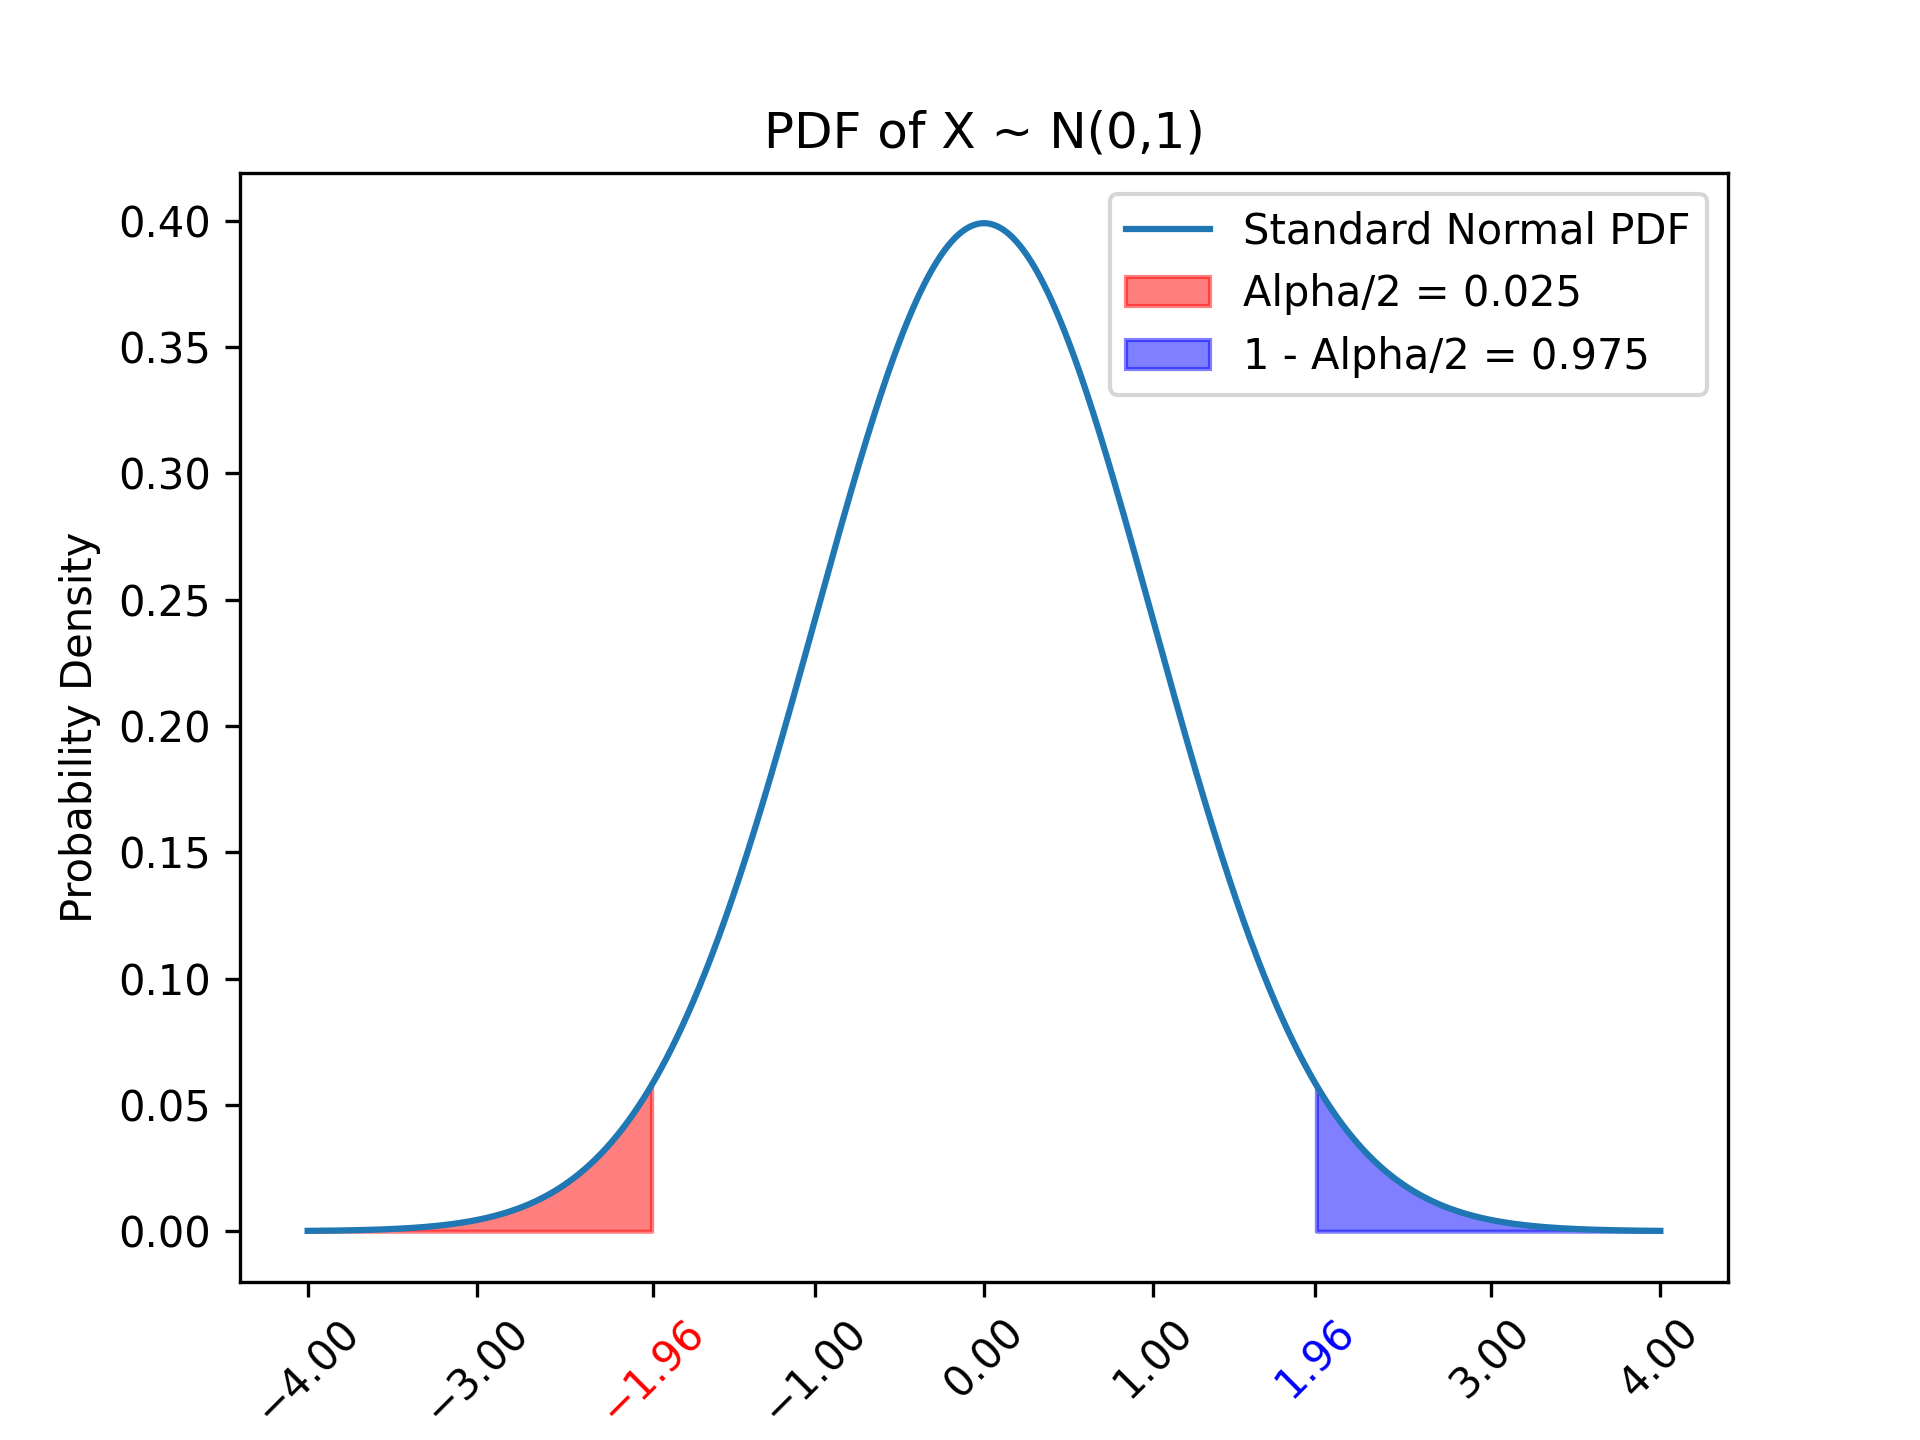
\includegraphics[width=\linewidth]{images/standard_normal_pdf.png}
	\caption{A visualization of the Normal Distribution's symmetric quantiles}
	\label{fig:standard_normal_pdf}
\end{figure}

\subsection{Sets of Related Random Variables}

Suppose we have two rvs $X$ and $Y$. We can define the \textbf{joint distribution} $p(x,y) = p(X = x, Y= y)$. If  $X$ and $Y$ have finite cardinality, one can represent their joint distribution in a 2D table:

\begin{table}[H]
	\centering
	\caption{Joint Distribution of Two Binary Random Variables $X$ and $Y$}
	\begin{tabular}{|c|c|c|c|}
		\hline
		& $Y = 0$ & $Y =  1$  \\ \hline
		$X = 0$ & $0.3$  & $0.2$  \\ \hline
		$X = 1$ & $0.2$ & $0.3$ \\ \hline
	\end{tabular}
\end{table}

If we are interested in only one of the variables distribution, i.e., we want one of the varibles \textbf{marginal}, we can use the follwing rule:

\begin{definition}[Sum Rule/ Rule of Total Probability]
	\label{def:sum_rule}
	
	Given a joint distribution function  $p(x,y)$, the marginal $p(x)$ is given by:
 	
	\begin{align}
		p(x) &= \sum_{i = 1}^{n} p(x, Y = y_i)
	\end{align}
	
\end{definition}

The marginal for $y$ (i.e., $p(y)$) is defined exactly the same way.

If $X$ and $Y$ are independent variables, which is written as $X \perp Y$, then  $p(x,y)$ can be defined as the product of the marginals.

\begin{definition}[Joint Distribution of Independent Random Variables]
	\label{def:joint_dist_of_indep_rvs}
	
	If $X$ and $Y$ are two independent random variables, which is written like  $X \perp Y$ then:
	
	\begin{align}
		p(x,y) &= p(x)p(y)\\
		& \text{which is a product of two vectors}
	\end{align}
	
\end{definition}

On the other hand, is far more common that variables are indeed dependent on each other, so that the definition above cannot be used to define their joint distribution. Hence, we use the $product rule$ instead:


\begin{definition}[Product Rule]
	\label{def:prod_rule}
	
	If $X$ and $Y$ are two random variables, then the product rule says that their joint distribution is given by:
	
	\begin{align}
		p(x,y) &= p(x)p(y|x)\\
	\end{align}
	
\end{definition}


We might generalize the joint distribution even further for the cases in which we have a set of random variables and we are interested to study their simultaneous behavior.

\begin{definition}[Chain Rule of Probability]
	\label{def:cahin_rule_prob}
	
	Given a set of $D$ random variables denoted by $X_1, X_2, \hdots, X_D$, one can define their joint distribution like the following:
	
	\begin{align}
		p(x_{1:D}) &= p(x)p(x_2|x_1)p(x_3| x_2, x_1)\hdots p(x_D|x_{D-1}, \hdots, x_1)\\
	\end{align}
	
\end{definition}
%------------------------------------------------

A set of random variables $X_1, \hdots, X_D$ is said to be \textbf{mutually independent} if the joint distribution for any subset $\{X_1, \hdots, X_m\}\subseteq \{X_1, \hdots, X_D\}$ can be written as a product of the marginals.

\begin{definition}[Mutual Independence]
	\label{def:mututal_indep}
	
	A set of $D$ random variables $\{X_1, X_2, \hdots, X_D\}$, is said to be mutually independent iff:
	
	\begin{align}
		p(x_1, x_2, \hdots, x_m) = p(x_{1:m}) &= p(x_1)p(x_2)\hdots p(x_m)\\
		&\text{for any  } m \leq D
	\end{align}
	
\end{definition}

As previously mentioned, a set of variables is rarely mutually independent, which means that the \textbf{chain rule of probability} is usually used to calculate joint distributions of their subsets. Intuitivelly, what this means is that it is very common that one variable influences one-another in a set of rvs. On the other hand, one can often describe $X$'s influence on $Y$ by using another rv $Z$ that medidates the influence such that the $X$ and $Y$  become \textbf{conditionally independent}.

\begin{definition}[Conditional Independence]
	\label{def:cond_indep}
	
	$X$ and $Y$ are said to be \textbf{conditionally independent} on $Z$, which is denoted by $X \perp Y | Z$, iff:
	
	\begin{align}
		p(X = x, Y=y | Z = z) &= p(x | z) p(y | z)
	\end{align}
	
\end{definition}


\subsection{Bayes' Rule}


\begin{definition}[Bayes Rule]
	\label{def:bayes_rule}
	
	The Bayes' Rule is simply a formula for computing the distribution of a hidden state $H$ given some observed data $Y$ :
	
	\begin{align}
		p(H = h | Y = y) &= \frac{p(Y = y | H = h) p(H = h)}{p(Y=y)}
	\end{align}
	
	This follows directly from the previously defined product rule (\ref{def:prod_rule}).
	
\end{definition}

There are some important names for the terms of the Bayes' Rule formula:

\begin{itemize}
	\item $p(H = h | Y = y)$:  is called the \textbf{posterior distribution}, because it is the distribution of $H$ after observing a certain value of $Y$.
	\item $p(Y = y | H = h)$: is called the \textbf{likelihood} and is a function of $h$ since $y$ is fixed. It measures how likely it is for $Y = y$ given that $H = h$. Notice this is not a probability distribution because it does not sum up to $1$ for all the differen values of $h$.
	\item $p(H = h)$: is called the \textbf{prior} distribution and is simply the distribution of $H$ before any knowledge about $Y$ is given.
	\item $p(Y = y)$: is called the \textbf{marginal likelihood} and can be calculated using the \textbf{sum rule/rule of total probability}, since $p(Y = y) = \sum_{i = 1}^{n} p(y, H = h_i)$.
\end{itemize}


\begin{info} % Information block
	We call \textbf{Bayesian Inference} the act of passing from sample data to generalizations (inference) with calculations of certainty given by the \textit{Bayes' Rule}. Hence, when we perform this type of inference, we use a set of observed samples (training set) to tell the shape of the posterior distribution of a variable of interest $H$ as a means to be able to qualify its possible outcomes quantitatively in terms of probabilities given an observation of the world $Y = y$.
\end{info}





\subsubsection{The Monty Hall Problem}

\begin{question}
	Suppose there is a contestant in a TV show in which there is a hidden prize behind only one of three distinct doors. In the beggining of the show, the contestant must choose one of the three doors and as soon as this choice is made, the host opens one of the remaining two doors \textbf{without revealing the prize location}. After such door is opened, the contestant must make a last choice: to keep their first door as the final choice or two switch it by the door that has not been opened by the host. \textbf{Which last choice maximixes the probability that the contestant wins the final prize?}
	
	To solve this problem, we first need to model it. Let's say the contestant first selects door $1$. Let's define some variables.
	
	\begin{itemize}
		\item  $C = c $ is the event when the contestant selects door $c$ at the end, $i \in \{1,2,3\}$
		\item  $H = h$ is the event when the TV host selects door $h \in \{1,2,3\}$
		\item $Y = y$ is the event when the prize is behind door $y \in \{1,2,3\}$
		\item $p(Y = y | H = h)$ is the probability we are interested to maximize. This means we want to the contestant to make a final choice for the door $y$ that is the most likely to have the prize given that the host selected door $h$.
	\end{itemize}
	
	Suppose $C = 1$. We can skip the calculation for $p(Y = y | H = c)$ and $p(Y = y | H = y)$, because they are certainly undefined and equal to $0$, respectively. This leaves us with:
	
	\begin{align}
		 p(Y = 1 | H = 2) &= \frac{p(H = 2 | Y = 1) p(Y = 1)}{p(H = 2)} = \frac{(1/2) (1/3)}{(1/2)} = 1/3 \\
		 p(Y = 1 | H = 3) &= \frac{p(H = 3 | Y = 1) p(Y = 1)}{p(H = 3)} = \frac{(1/2) (1/3)}{(1/2)} = 1/3 \\
		 p(Y = 2 | H = 3) &= \frac{p(H = 3 | Y = 2) p(Y = 2)}{p(H = 3)} = \frac{(1) (1/3)}{(1/2)} = 2/3 \\
		 p(Y = 3 | H = 2) &= \frac{p(H = 2 | Y = 3) p(Y = 3)}{p(H = 2)} = \frac{(1) (1/3)}{(1/2)} = 2/3 \\
	\end{align}
	
	Above, we see that $p(Y = 2 | H = 3)$ and $p(Y = 3 | H = 2)$ are the posteriors with the largest values. They are modeling the probability that the prize is behind the door that has not been chosen by either the TV host or by the contestant at the begining, which is $C = 1$. The initial choice of $C=1$ is irrelevant here and what matters is that changing the choice of the door yelds the maximum probability of winning the prize.  \textbf{Hence, the contestant should switch their choice after the host opens a door as it will lead to the event in which the probability of winning is the largest. }
\end{question}




\subsection{The Univariate Normal Distribution}


\subsubsection{Cumulative Distribution  Function ($\mathbf{cdf}$)}

It is the function that tells the probability of a normally distributed random variable $\mathbf{Y}$ to be observed inside a specific interval.

\begin{definition}[Univariate Gaussian Cumulative Distribution  Function ($\mathbf{cdf}$)]
	\begin{align}
		p(y_1 \leq Y  \leq y_2) &=  \int_{y_1}^{y_2}  \mathcal{N}(y; \mu, \sigma^2) \, dy \\
											   &= p(y_2) - p(y_1)
	\end{align}
\end{definition}


\begin{definition}[Univariate Gaussian Probability Density  Function ($\mathbf{pdf}$)]
	\begin{align}
		p(Y = y) &=  \mathcal{N}(y; \mu, \sigma^2) \\
					   &= \frac{1}{\sqrt{2\pi\sigma^2}}e^{-\frac{1}{2\sigma^2}(y - \mu)^2}
	\end{align}
\end{definition}

In the $\mathbf{pdf}$ of the univariate gaussian, $\sqrt{2\pi\sigma^2}$ is the normalization constant that ensures that the $\mathbf{cdf}$ equals to $1$.

\subsubsection{Percent Point Function ($\mathbf{ppf}$)/ Probit  Function/ Inverse of $\mathbf{cdf}$/ The quantile }

The output of this function tells the observation  $y$ for which its cumulative distribution ($\mathbf{cdf}$) is equal to the input $z$. In other words, $\mathbf{ppf(z)} = y \text{  iff  }  \mathbf{cdf(y)} = z$.

For example, if $\mathbf{ppf(0.5)} = y_0$ for a normally distributed rv $Y = y$, then it means that $50\%$ of the observations of $Y$ are less or equal to $y_0$.


\subsection{The Binomial Distribution}

It is a distribution that models a sequence of independent binary events. The rv distributed as a $binomial$ basically tells how much of the events in the sequence was a positive.

\begin{definition}[Binomial Distribution]
	
	Let $Y  ~ Bin(\theta, N)$ where $N$ is the sequence length, i.e., the number of bianary events. Hence:
	\begin{align}
		P(Y = y) &= \binom{N}{s}\theta^s(1 - \theta)^{N-s}\\
		E(Y) &= N\theta \\
		Var(Y) &= N\theta(1 - \theta) 
	\end{align}
	
	This is so, because $p(Y = y) = \theta$ and we are dealing with a binary event, so there is a $\theta$ probability that the event is positive among $N$ observations.
\end{definition}

\subsubsection{The Bernoulli Distribution}
The Bernoutlli distribution is denoted by $Ber(\theta)$ and it is a special case of the binomial distribution in which the sequence of events hs length $1$. Hence:

\begin{definition}[Bernoulli Distribution]
	
	Let $Y  ~ Ber(\theta)$.
	\begin{align}
		p(Y = y) = 
		\begin{cases} 
			\theta & y =  1 \\
			1 -  \theta & y = 0 \\
		\end{cases}
		&= Bin(1, \theta)
	\end{align}
\end{definition}
This is so, because $p(Y = y) = \theta$ and we are dealing with a binary event, so there is a $\theta$ probability that the event is positive among $N$ observations.


\subsection{The Poisson Distribution}

It is a distribution for discrete rv's that account the number of binary events in a fixed period of time under the following assumptions:

\begin{itemize}
	\item The events in a given period of time are independent of each other
	\item The average number of positive events in a given period of time is fixed regardless of the beginning of the period
\end{itemize}

\begin{definition}[Poisson Distribution]
	Let $ Y ~ Poisson(\lambda)$, where $\lambda$ is the average number of positive events in a given period of time. Hence:
	
	\begin{align}
		p(Y = y) & = \frac{\lambda^ye^{-\lambda}}{y!} \\
		E(Y) &= Var(Y) = \lambda
	\end{align}
\end{definition}

The expected value and the variance of a poisson distributed rv are equal to the mean number of positive events in a given period of time, i.e., $\lambda$.

The Poisson Distribution closely approximates the Binomial Distributions for large values of $N$ and small values of $\theta$. For example, the distribution of the number of decayed atoms in a set of atoms in a fixed period of time can be assumed to be a Poisson distribution where $\lambda$ is the average number of atoms that decay in the same period of time. On the other hand, such number $N$ of atoms is very large and the probability of a single one to decay is small, so one can approximate the  number $s$ of atoms that decay in the same period of time as a Binomial Distribution.


\subsection{The Geometric Distribution}

It is a distribution for discrevete rv's that counts the number of Bernoulli trials until the first positive event happens.

\begin{definition}[Geometric Distribution]
	Let $ Y ~ Geo(\theta)$, where $\theta$ is the probability of sucess.
	\begin{align}
		p(Y = y) & = \theta^{y -1}(1 - \theta) \\
		E(Y) &= \frac{1}{\theta} \\
		Var(Y) &= \frac{1 - p}{p ^2}
	\end{align}
\end{definition}

\subsection{What Properties Should Sinusoidal Embeddings (SE) Should Apply?}

\begin{enumerate}
	\item \textbf{Periodicity:} the model trained with sinusoidal embeddings should be able to capture the relative positions of tokens effectively, which means that the distances between the embeddings of a pair of clauses should not depend on their absolute position within the longer sentence. This is achieved by making the sinusoidal embeddings functions periodic, which was to be expected from the name of the function. 
	\item \textbf{Unique Representation (Injective Function):} this one is straight forward from the fact that  sinusoidal embeddings must represent the positions of tokens within a sentence. This means that sets of tokens in different positions should not be mapped to the same output, otherwise different positions would have the same representation.
	\item \textbf{Scale Invariance:} sinusoidal embeddings should represent tokens positions consistently regardless of the sequence length. This property is crucial for handling sequences of varying lengths in a transformer model including those that are longer than the ones the model were trained on. Essentialy, the scale invariance property says that the distance of two inputs $x_t$ and $x_{t - k}$ should be similar among different values of $t$. In other words, $x_t - x_{t - k}$ should not depend on $t$.
	\item \textbf{Linearity:} this property is somewhat related to the scale invariance property. For the Sinusoidal Embedding function to be linear is good, because functions having such property are more easily learned by neural networks. Moreover, if the Sinusoidal Embedding Function is linear we also achieve the scale invariance property. This is true, because if such Sinusoidal Embedding function ($SE$) is linear, for any pair of sets of tokens separated by a distance of $k$, say $X_t, X_{t+k}$, there is a linear transformation $M$ such that $M \times SE(X_t) = SE(X_{t+k})$. Hence, in order to represent $X_{t+k}$,  the model must only learn the linear transformation $M$ regardless of the value of $k$. 
\end{enumerate}


\subsection{How are Sinusoidal Embeddings Defined?}

The author's of the \textit{Attention is All You Need} paper define the Sinusoidal Embeddings Function ($SE$) like the following.

\begin{definition}[Sinusoidal Embeddings]
	\label{def:sin_embedding}
	
	For a position \( pos \) in the sequence and a dimension \( i \) (where \( i \) ranges from 0 to \( \frac{d}{2}-1 \)), the embedding is given by:
	
	\begin{align}
		SE_{(pos, 2i)} &= \sin\left(\frac{pos}{10000^{\frac{2i}{d}}}\right) \\
		SE_{(pos, 2i+1)} &= \cos\left(\frac{pos}{10000^{\frac{2i}{d}}}\right) \\
	\end{align}
	
	This function can be vectorially expressed as the following: 
	\begin{align}
		\mathbf{SE}(pos) &= \left[ \sin\left(pos \cdot e^{- \frac{2i \ln(10000)}{d}}\right), \cos\left(pos \cdot e^{- \frac{2i \ln(10000)}{d}}\right) \right]_{i=0}^{\frac{d}{2}-1}
	\end{align}
	

\end{definition}

where:

\begin{itemize}
	\item \( pos \) is the position in the sequence.
	\item  \( i \) is the dimension index.
	\item  \( d \) is the dimensionality of the embeddings.
\end{itemize}


Notice that $SE$ is essentialy a function that outputs $sin$ values to the even dimensions of an input $x_t$ and $cos$ for the odd ones with exponentially decreasing frequencies.


In the next section we will use the definition of  $SE$ function to verify the validity of the previous $4$ properties it should have. Some verification will be done analitically and others will be done using $Python$.

\section{Properties Verification}

In this section, we will be checking each of the $4$ presented properties of the Sinusoidal Embeddings using analytical techniques.


\subsection{Peridiocity}

This peridiocity of the $SE$ function is straight-forward. Different dimensions $i$ and $i+k$ of an input  $x_t \in \mathbb{R}^{d}$ with position $pos$ will have the same values output by the $sin$ and $cos$ because such functions are periodic. 

\begin{info} % Information block
	One question that a reader might have is whether the peridiocity property does not contradict the injectivity one. The answer for that is no. The peridiocity property is observed at a single dimension level, which means $SE_{(pos, 2i)}$ that outputs a single value, is be periodic. The injectivity, on the other hand, is observed at the entire embedding level, which means $SE_{(pos)}$, that outputs a vector (embedding) of dimension $d$ is injective.
\end{info}


\subsection{Unique Representation (Injective Function)}

We are gonna prove that two sequences from different positions are \textbf{not} mapped to the same vector/output, using a \textit{proof by contradiction}. 
Let's assume that two sequences $x_{t_1}$ and $x_{t_2}$, with different positions $t_1$ and $t_2$, respectivelly, are mapped to the same output using the previously  $SE$ function. This assumption implies the following \textbf{for any dimension i}

\begin{align}
	SE(x_{t_1}) = SE(x_{t_2}) & \implies SE(t_1, 2i) = SE(t_2, 2i) \text{   and   }SE(t_1, 2i+1) = SE(t_2, 2i+1) \\
	 \implies \sin\left(\frac{t_1}{10000^{\frac{2i}{d}}}\right) &= \sin\left(\frac{t_2}{10000^{\frac{2i}{d}}}\right) \text{   and   }\cos\left(\frac{t_1}{10000^{\frac{2i}{d}}}\right) = \cos\left(\frac{t_2}{10000^{\frac{2i}{d}}}\right) 
\end{align}


For the last implication to be true, either the arguments of the $sin$ and $cos$ functions are the exact same or they are separated by $2\pi k$. We know they are not the same, because $t_1 \neq t_2$. Therefore, we're left with the condition:


\begin{align}
	| \frac{t_1}{10000^{\frac{2i}{d}}} - \frac{t_2}{10000^{\frac{2i}{d}}} | &=  2\pi k \\
	\implies 	| \frac{t_1 - t_2}{10000^{\frac{2i}{d}}} | &=  2\pi k \\
	\implies 	| t_1 - t_2 | &=  2\pi k 10000^{\frac{2i}{d}} \\
\end{align}


Since \( t_1 \) and \( t_2 \) are integers that represent the sequences positions, and \( 10000^{\frac{2i}{d}} \) is a positive real number, the right side of the equation \( \left| t_1 - t_2 \right| = 2\pi k \cdot 10000^{\frac{2i}{d}} \) must also be an integer. However, \( 2\pi k \cdot 10000^{\frac{2i}{d}} \) is generally not an integer because \( 2\pi \) is an irrational number, which leads us to a contradiction.

Hence, the initial assumption $SE(x_{t_1}) = SE(x_{t_2})$ must be false, which let's us say that \textbf{ two sequences $x_{t_1}$ and $x_{t_2}$, with different positions $t_1$ and $t_2$, respectivelly, are not mapped to the same output using the previously  $SE$ function}.


\subsection{Linearity \& Scale Invariance}

As previously mentioned, the scale invariance property is a consequence of $SE(pos)$'s linearity. Hence, by proving that $SE(pos)$ is linear we also prove that such function is scale invariant. 

We need to find $M \in \mathbb{R}^{d \times d}$ such that $M \times  SE(x_{t}) = SE(x_{t + k}) $. We have the following system of equations:

\begin{align}
	\begin{bmatrix}
		m_{00} & m_{01} & \cdots & m_{0(d-1)} \\
		m_{10} & m_{11} & \cdots & m_{1(d-1)} \\
		\vdots & \vdots & \ddots & \vdots \\
		m_{(d-1) 0} & m_{(d-1)1} & \cdots & m_{(d-1)(d-1)}
	\end{bmatrix}
	\begin{bmatrix}
		sin(\omega_0 t) \\
		cos(\omega_0 t) \\
		\vdots \\
		sin(\omega_{(d-2)/2} t) \\
		cos(\omega_{(d-2)/2} t) 
	\end{bmatrix}
	&=\begin{bmatrix}
		sin(\omega_0 (t+k)) \\
		cos(\omega_0 (t+k)) \\
		\vdots \\
		sin(\omega_{(d-2)/2}  (t+k)) \\
		cos(\omega_{(d-2)/2} (t+k)) 
	\end{bmatrix}
\end{align}

\begin{align}
	m_{00}\sin(\omega_0 t) + m_{01}\cos(\omega_0 t) + \cdots + m_{0(d-1)}\cos(\omega_{d-1} t) &= \sin(\omega_0 t)\cos(\omega_0 k) + \sin(\omega_0 k)\cos(\omega_0 t) \\
	m_{10}\sin(\omega_0 t) + m_{11}\cos(\omega_0 t) + \cdots + m_{1(d-1)}\cos(\omega_{d-1} t) &= \cos(\omega_0 t)\cos(\omega_0 k) - \sin(\omega_0 k)\sin(\omega_0 t) \\
	&\vdots \nonumber \\
	m_{(d-1)0}\sin(\omega_0 t) + m_{(d-1)1}\cos(\omega_0 t) + \cdots + m_{(d-1)(d-1) }\cos(\omega_{(d-2)/2}  t) &= \cos(\omega_{(d-2)/2}  t)\cos(\omega_{(d-2)/2}  k) - \sin(\omega_{(d-2)/2}  k)\sin(\omega_{(d-2)/2}  t)
\end{align}


This system has a solution:
\begin{align}
	m_{00} &= \cos(\omega_0 k) \\
	m_{01} &= \sin(\omega_0 k) \\
	m_{02} &= m_{03} = \hdots = m_{0(d-1)} = 0 \\
	m_{10} &= -\sin(\omega_0 k) \\
	m_{11} &= \cos(\omega_0 k) \\
	m_{12} &= m_{13} = \hdots = m_{1(d-1)} = 0 \\
	m_{22} &= \cos(\omega_1 k) \\
	m_{23} &= \sin(\omega_1 k) \\
	m_{20} &= m_{21} = m_{24} = \hdots = m_{2(d-1)} = 0 \\
	m_{32} &= -\sin(\omega_1 k) \\
	m_{33} &= \cos(\omega_1 k) \\
	m_{30} &= m_{31} = m_{34} = \hdots = m_{3(d-1)} = 0 \\
	& \vdots \nonumber \\
	m_{(d-2)(d-2)} &= \cos(\omega_{(d-2)/2} k) \\
	m_{(d-2)(d-1)} &= \sin(\omega_{(d-2)/2} k) \\
	m_{(d-2)0} &= m_{(d-2)1} = m_{(d-2)2} = \hdots = m_{(d-2)(d-3)} = 0 \\
	m_{(d-1)(d-2)} &= -\sin(\omega_{(d-2)/2} k) \\
	m_{(d-1)(d-1)} &= \cos(\omega_{(d-2)/2} k) \\
	m_{(d-1)0} &= m_{(d-1)1} = m_{(d-1)2} = \hdots = m_{(d-1)(d-3)} = 0 \\
\end{align}

Which lets us define $M$ as:

\begin{align}
	M &=
	\begin{bmatrix}
		\cos(\omega_0 k) & \sin(\omega_0 k) & 0 & 0 & \cdots & 0 & 0 \\
		-\sin(\omega_0 k) & \cos(\omega_0 k) & 0 & 0 & \cdots & 0 & 0 \\
		0 & 0 & \cos(\omega_1 k) & \sin(\omega_1 k) & \cdots & 0 & 0 \\
		0 & 0 & -\sin(\omega_1 k) & \cos(\omega_1 k) & \cdots & 0 & 0 \\
		\vdots & \vdots & \vdots & \vdots & \ddots & \vdots & \vdots \\
		0 & 0 & 0 & 0 & \cdots & \cos(\omega_{(d-2)/2} k) & \sin(\omega_{(d-2)/2} k) \\
		0 & 0 & 0 & 0 & \cdots & -\sin(\omega_{(d-2)/2} k) & \cos(\omega_{(d-2)/2} k)
	\end{bmatrix}
\end{align}



We found a matrix $M \in \mathbb{R}^{d \times d}$ such that $M \times  SE(x_{t}) = SE(x_{t + k}) $. Hence, $SE$ is a linear function. Moreover, notice how \textbf{M does not depend on t}, only on $k$. This is what gives us the scale invariability property.

\section{Visualizing the Sinuspoidal Embeddings Properties With \textit{Python}}

In this section, we will write some $Python$ functions and classes to visualize the $4$ cited properties of Sinusoidal Embeddings. Visualization is a great way to grasp such function's behaviour without having to necessarily prove it (even though you can always come back to this post with you're interested in the proofs).

\subsection{Sinusoidal Embedding Definition With Pytorch}

The sinusoidal embeddings module will store a multi-embedding tensor with $shape =  (max\_pos, embed\_dim)$, where $max\_pos$ represents the maximum position we are interested in representing. This way, each of such tensor's row represents a the sinusoidal embedding for a position $pos$ such that $SE(pos), 0 \leq pos <  max\_pos $. 


\begin{lstlisting}[caption={Sinusoidal Embedding Module Definition}]
	
import pytorch.nn as nn
	
class SinusoidalEmbeddings(nn.Module):

	def __init__(self, max_pos:int, embed_dim: int):
		super().__init__()
		# Returns a tensor with shape (time_steps, 1).
		positions = torch.arange(max_pos).unsqueeze(1).float()
		
		# Creates a tensor with shape (embed_dim //2,). We just need 
		# half of the dimensions of the input embeddings to compute all
		# of the sinusoidal embeddings frequencies
		dimensions = torch.arange(start = 0, end = embed_dim, step = 2).float()
		
		# Compute the frequencies vector
		frequencies = torch.exp(dimensions * -(math.log(10000.0) / embed_dim))
		
		# Initialize the embeddings tensor with shape (time_steps, embed_dim)
		embeddings = torch.zeros(time_steps, embed_dim, requires_grad=False)
		
		# Apply sin to even indices (0, 2, 4, ...) of the input embeddings
		embeddings[:, 0::2] = torch.sin(positions * frequencies)
		
		# Apply cos to odd indices (1, 3, 5, ...) of the input embeddings
		embeddings[:, 1::2] = torch.cos(positions * frequencies)
		
		self.embeddings = embeddings
	
	def forward(self, x, t):
		embeds = self.embeddings[t].to(x.device)
		return embeds[:, :, None, None]

\end{lstlisting}

\subsection{Sinusoidal Embeddings Periodicity}

As previously mentioned, the periodicity of  Sinusoidal Embeddings is observed in each of its dimensions. Hence, we need to plot its dimensions values for different positions to see their periodic behavior. 

\begin{lstlisting}[caption={Generating the plot of the embedding's dimensions for in different positions}]
	
max_pos = 100

# Our embeddings will only have 4 dimension
embed_dim = 4
sinusoidal_embeddings = SinusoidalEmbeddings(max_pos, embed_dim)

# Generate embeddings for a range of time steps
embeddings = sinusoidal_embeddings.embeddings

# Convert embeddings to numpy for plotting
embeddings_np = embeddings.numpy()

# Plot the sunosoidal embeddings for different time steps
plt.figure(figsize=(14, 8))
for i in range(embed_dim):
	plt.plot(embeddings_np[:, i], label=f"Dim {i} (i = {i//2})")
	
plt.title("SE(pos, 2i)")
plt.xlabel("pos")
plt.ylabel("Value")
plt.legend(loc="upper right", bbox_to_anchor=(1.15, 1))
\end{lstlisting}


As noticed in the plot above, the value of the function $SE(pos, 2i)$ defined in \ref{def:sin_embedding} repeats itself in a frequency that is inversely proportional to $i$, which is the dimension being represented (an index in the multidimensional embedding). As a consequence, \textbf{the higher the dimension of our model's embeddings (previously called $d$ and called $embed\_dim$ in the Sinusoidal Embedding module), the less $SE$ values vary.} 

Intuitively, such consequence means that embeddings close to each other (they represent sentences in not very distant positions), will have their differences captured in lower dimensions, because their higher dimensions are likely to be very similar. The exact opposite is true for embeddings that represent sentences that are far away from each other. Let's visualize that by plotting different embeddings' heatmaps.


\begin{lstlisting}[caption={Generating the plot of the sinusoidal embeddings for different positions}]
	
import torch

# We'll create embeddings with many dimensions to better see the 
# frequency decay effect
max_pos = 100
embed_dim = 128
sinusoidal_embeddings = SinusoidalEmbeddings(max_pos, embed_dim)

x = torch.zeros(embed_dim)
results = torch.zeros(max_pos, embed_dim)
for pos in range(max_pos):
results[pos] =  x + sinusoidal_embeddings.embeddings[pos]

tensor_np = results.numpy()
# Plot the heatmap using matplotlib
plt.figure(figsize=(16, 6))
plt.imshow(tensor_np, aspect='auto', cmap='RdBu')
plt.colorbar(label='')
plt.xlabel('2i')
plt.ylabel('pos')
plt.title('SE(pos, 2i)')
plt.show()
\end{lstlisting}


In the plot above, we see that embeddings with close positions (two close values in the $pos$ axis) have different values of $SE(pos, 2i)$ for very small $2i$ (lower dimensions) while their values for higher dimensions are similar. On the other hand, if we pick two embeddings with very distant $pos$, they might differ from each other only in higher dimension. What this means is that in order to represent longer sentences (that contain positions very distant from each other), our model needs to have more dimensions. \textbf{The longer the input sentences, the higher the model's dimensions need to be.}

\subsection{Unique Representativiness ($SE$ is an injective function)}

Figure \ref{fig:sin_embeds_freq_decay} shows us that no two rows are the same because of the exponential decay of the frequencies with the increase of the dimension (increase of $2i$). As each row represents embeddings with different positions, what the figure is essentialy showing us is that two embeddings with different positions will never have the same representation, i.e., $SE$ is injective.

\subsection{Linearity \& Scale Invariance}

As previously mentioned, to be scale invariant, $SE$ must be such that the distance between $SE(pos)$ and $SE(pos + k)$ must be the same as the one between $SE(0)$ and $SE(k)$. In order to check that, we'll calculate the distance between every two sinusoidal embeddings of our module and see the linear property of such distance. Hence, all the rows will have to be subtracted from the first one, from the second one and so on up until the last one. 


\begin{lstlisting}[caption={Generating the plot of the module of the difference between every two different positions sinusoidal embeddings}]
	
import torch

# We'll create embeddings with many dimensions to better see the 
# frequency decay effect
max_pos = 1000
embed_dim = 1000


sinusoidal_embeddings = SinusoidalEmbeddings(max_pos, embed_dim).embeddings

# A single column tensor where each row's single element contains an 
# entire sinusoidal embeddings tensor
T_2 = sinusoidal_embeddings[:, None, :]

# A single row tensor where column's single element contains an 
# entire sinusoidal embeddings tensor
T_1 = sinusoidal_embeddings[None, :, :]

# By broadcasting, this operation will save the desired differences
# in the tensor's last dimension
differences = T_2 - T_1

# As the differences were saved in the last dimension, we need 
# to calculate the norm with respect to it, which is indicated 
# by dim=-1
distances = torch.norm(differences, p=2, dim=-1)

# Plot the resulting 2D tensor as a heatmap
plt.figure(figsize=(8, 6))
plt.imshow(distances.numpy(), aspect="auto", cmap="PuRd")
plt.colorbar(label="L2 Norm (Euclidean Distance)")
plt.xlabel("pos")
plt.ylabel("pos")
plt.title("Euclidean Distances Between Different Position Sinusoidal Embeddings")
plt.show()


\end{lstlisting}
Figure \ref{fig:sin_embeds_scale_invariance} above shows us how the distance between sinusoidal embeddings of different positions decreases smoothly and linearly for embedidding with $d = 1000$.

\begin{question}
	Quisque ullamcorper placerat ipsum. Cras nibh. Morbi vel justo vitae lacus tincidunt ultrices. Lorem ipsum dolor sit amet, consectetuer adipiscing elit.

	% Subquestions numbered with letters
	\begin{enumerate}[(a)]
		\item Do this.
		\item Do that.
		\item Do something else.
	\end{enumerate}
\end{question}
	
%------------------------------------------------

\subsection{Algorithmic issues}

In malesuada ullamcorper urna, sed dapibus diam sollicitudin non. Donec elit odio, accumsan ac nisl a, tempor imperdiet eros. Donec porta tortor eu risus consequat, a pharetra tortor tristique. Morbi sit amet laoreet erat. Morbi et luctus diam, quis porta ipsum. Quisque libero dolor, suscipit id facilisis eget, sodales volutpat dolor. Nullam vulputate interdum aliquam. Mauris id convallis erat, ut vehicula neque. Sed auctor nibh et elit fringilla, nec ultricies dui sollicitudin. Vestibulum vestibulum luctus metus venenatis facilisis. Suspendisse iaculis augue at vehicula ornare. Sed vel eros ut velit fermentum porttitor sed sed massa. Fusce venenatis, metus a rutrum sagittis, enim ex maximus velit, id semper nisi velit eu purus.

\begin{center}
	\begin{minipage}{0.5\linewidth} % Adjust the minipage width to accomodate for the length of algorithm lines
		\begin{algorithm}[H]
			\KwIn{$(a, b)$, two floating-point numbers}  % Algorithm inputs
			\KwResult{$(c, d)$, such that $a+b = c + d$} % Algorithm outputs/results
			\medskip
			\If{$\vert b\vert > \vert a\vert$}{
				exchange $a$ and $b$ \;
			}
			$c \leftarrow a + b$ \;
			$z \leftarrow c - a$ \;
			$d \leftarrow b - z$ \;
			{\bf return} $(c,d)$ \;
			\caption{\texttt{FastTwoSum}} % Algorithm name
			\label{alg:fastTwoSum}   % optional label to refer to
		\end{algorithm}
	\end{minipage}
\end{center}

Fusce varius orci ac magna dapibus porttitor. In tempor leo a neque bibendum sollicitudin. Nulla pretium fermentum nisi, eget sodales magna facilisis eu. Praesent aliquet nulla ut bibendum lacinia. Donec vel mauris vulputate, commodo ligula ut, egestas orci. Suspendisse commodo odio sed hendrerit lobortis. Donec finibus eros erat, vel ornare enim mattis et.

% Numbered question, with an optional title
\begin{question}[\itshape (with optional title)]
	In congue risus leo, in gravida enim viverra id. Donec eros mauris, bibendum vel dui at, tempor commodo augue. In vel lobortis lacus. Nam ornare ullamcorper mauris vel molestie. Maecenas vehicula ornare turpis, vitae fringilla orci consectetur vel. Nam pulvinar justo nec neque egestas tristique. Donec ac dolor at libero congue varius sed vitae lectus. Donec et tristique nulla, sit amet scelerisque orci. Maecenas a vestibulum lectus, vitae gravida nulla. Proin eget volutpat orci. Morbi eu aliquet turpis. Vivamus molestie urna quis tempor tristique. Proin hendrerit sem nec tempor sollicitudin.
\end{question}

Mauris interdum porttitor fringilla. Proin tincidunt sodales leo at ornare. Donec tempus magna non mauris gravida luctus. Cras vitae arcu vitae mauris eleifend scelerisque. Nam sem sapien, vulputate nec felis eu, blandit convallis risus. Pellentesque sollicitudin venenatis tincidunt. In et ipsum libero. Nullam tempor ligula a massa convallis pellentesque.

%----------------------------------------------------------------------------------------
%	PROBLEM 2
%----------------------------------------------------------------------------------------

\section{Implementation}

Proin lobortis efficitur dictum. Pellentesque vitae pharetra eros, quis dignissim magna. Sed tellus leo, semper non vestibulum vel, tincidunt eu mi. Aenean pretium ut velit sed facilisis. Ut placerat urna facilisis dolor suscipit vehicula. Ut ut auctor nunc. Nulla non massa eros. Proin rhoncus arcu odio, eu lobortis metus sollicitudin eu. Duis maximus ex dui, id bibendum diam dignissim id. Aliquam quis lorem lorem. Phasellus sagittis aliquet dolor, vulputate cursus dolor convallis vel. Suspendisse eu tellus feugiat, bibendum lectus quis, fermentum nunc. Nunc euismod condimentum magna nec bibendum. Curabitur elementum nibh eu sem cursus, eu aliquam leo rutrum. Sed bibendum augue sit amet pharetra ullamcorper. Aenean congue sit amet tortor vitae feugiat.

In congue risus leo, in gravida enim viverra id. Donec eros mauris, bibendum vel dui at, tempor commodo augue. In vel lobortis lacus. Nam ornare ullamcorper mauris vel molestie. Maecenas vehicula ornare turpis, vitae fringilla orci consectetur vel. Nam pulvinar justo nec neque egestas tristique. Donec ac dolor at libero congue varius sed vitae lectus. Donec et tristique nulla, sit amet scelerisque orci. Maecenas a vestibulum lectus, vitae gravida nulla. Proin eget volutpat orci. Morbi eu aliquet turpis. Vivamus molestie urna quis tempor tristique. Proin hendrerit sem nec tempor sollicitudin.

% File contents
\begin{file}[hello.py]
\begin{lstlisting}[language=Python]
#! /usr/bin/python

import sys
sys.stdout.write("Hello World!\n")
\end{lstlisting}
\end{file}

Fusce eleifend porttitor arcu, id accumsan elit pharetra eget. Mauris luctus velit sit amet est sodales rhoncus. Donec cursus suscipit justo, sed tristique ipsum fermentum nec. Ut tortor ex, ullamcorper varius congue in, efficitur a tellus. Vivamus ut rutrum nisi. Phasellus sit amet enim efficitur, aliquam nulla id, lacinia mauris. Quisque viverra libero ac magna maximus efficitur. Interdum et malesuada fames ac ante ipsum primis in faucibus. Vestibulum mollis eros in tellus fermentum, vitae tristique justo finibus. Sed quis vehicula nibh. Etiam nulla justo, pellentesque id sapien at, semper aliquam arcu. Integer at commodo arcu. Quisque dapibus ut lacus eget vulputate.

% Command-line "screenshot"
\begin{commandline}
	\begin{verbatim}
		$ chmod +x hello.py
		$ ./hello.py

		Hello World!
	\end{verbatim}
\end{commandline}

Vestibulum sodales orci a nisi interdum tristique. In dictum vehicula dui, eget bibendum purus elementum eu. Pellentesque lobortis mattis mauris, non feugiat dolor vulputate a. Cras porttitor dapibus lacus at pulvinar. Praesent eu nunc et libero porttitor malesuada tempus quis massa. Aenean cursus ipsum a velit ultricies sagittis. Sed non leo ullamcorper, suscipit massa ut, pulvinar erat. Aliquam erat volutpat. Nulla non lacus vitae mi placerat tincidunt et ac diam. Aliquam tincidunt augue sem, ut vestibulum est volutpat eget. Suspendisse potenti. Integer condimentum, risus nec maximus elementum, lacus purus porta arcu, at ultrices diam nisl eget urna. Curabitur sollicitudin diam quis sollicitudin varius. Ut porta erat ornare laoreet euismod. In tincidunt purus dui, nec egestas dui convallis non. In vestibulum ipsum in dictum scelerisque.

% Warning text, with a custom title
\begin{warn}[Notice:]
  In congue risus leo, in gravida enim viverra id. Donec eros mauris, bibendum vel dui at, tempor commodo augue. In vel lobortis lacus. Nam ornare ullamcorper mauris vel molestie. Maecenas vehicula ornare turpis, vitae fringilla orci consectetur vel. Nam pulvinar justo nec neque egestas tristique. Donec ac dolor at libero congue varius sed vitae lectus. Donec et tristique nulla, sit amet scelerisque orci. Maecenas a vestibulum lectus, vitae gravida nulla. Proin eget volutpat orci. Morbi eu aliquet turpis. Vivamus molestie urna quis tempor tristique. Proin hendrerit sem nec tempor sollicitudin.
\end{warn}

%----------------------------------------------------------------------------------------

\end{document}
